\section{Implementation}
\label{sec:implementation}

\begin{figure*}[t]
    \centering
    \begin{subfigure}[b]{0.5\textwidth}
        \centering
        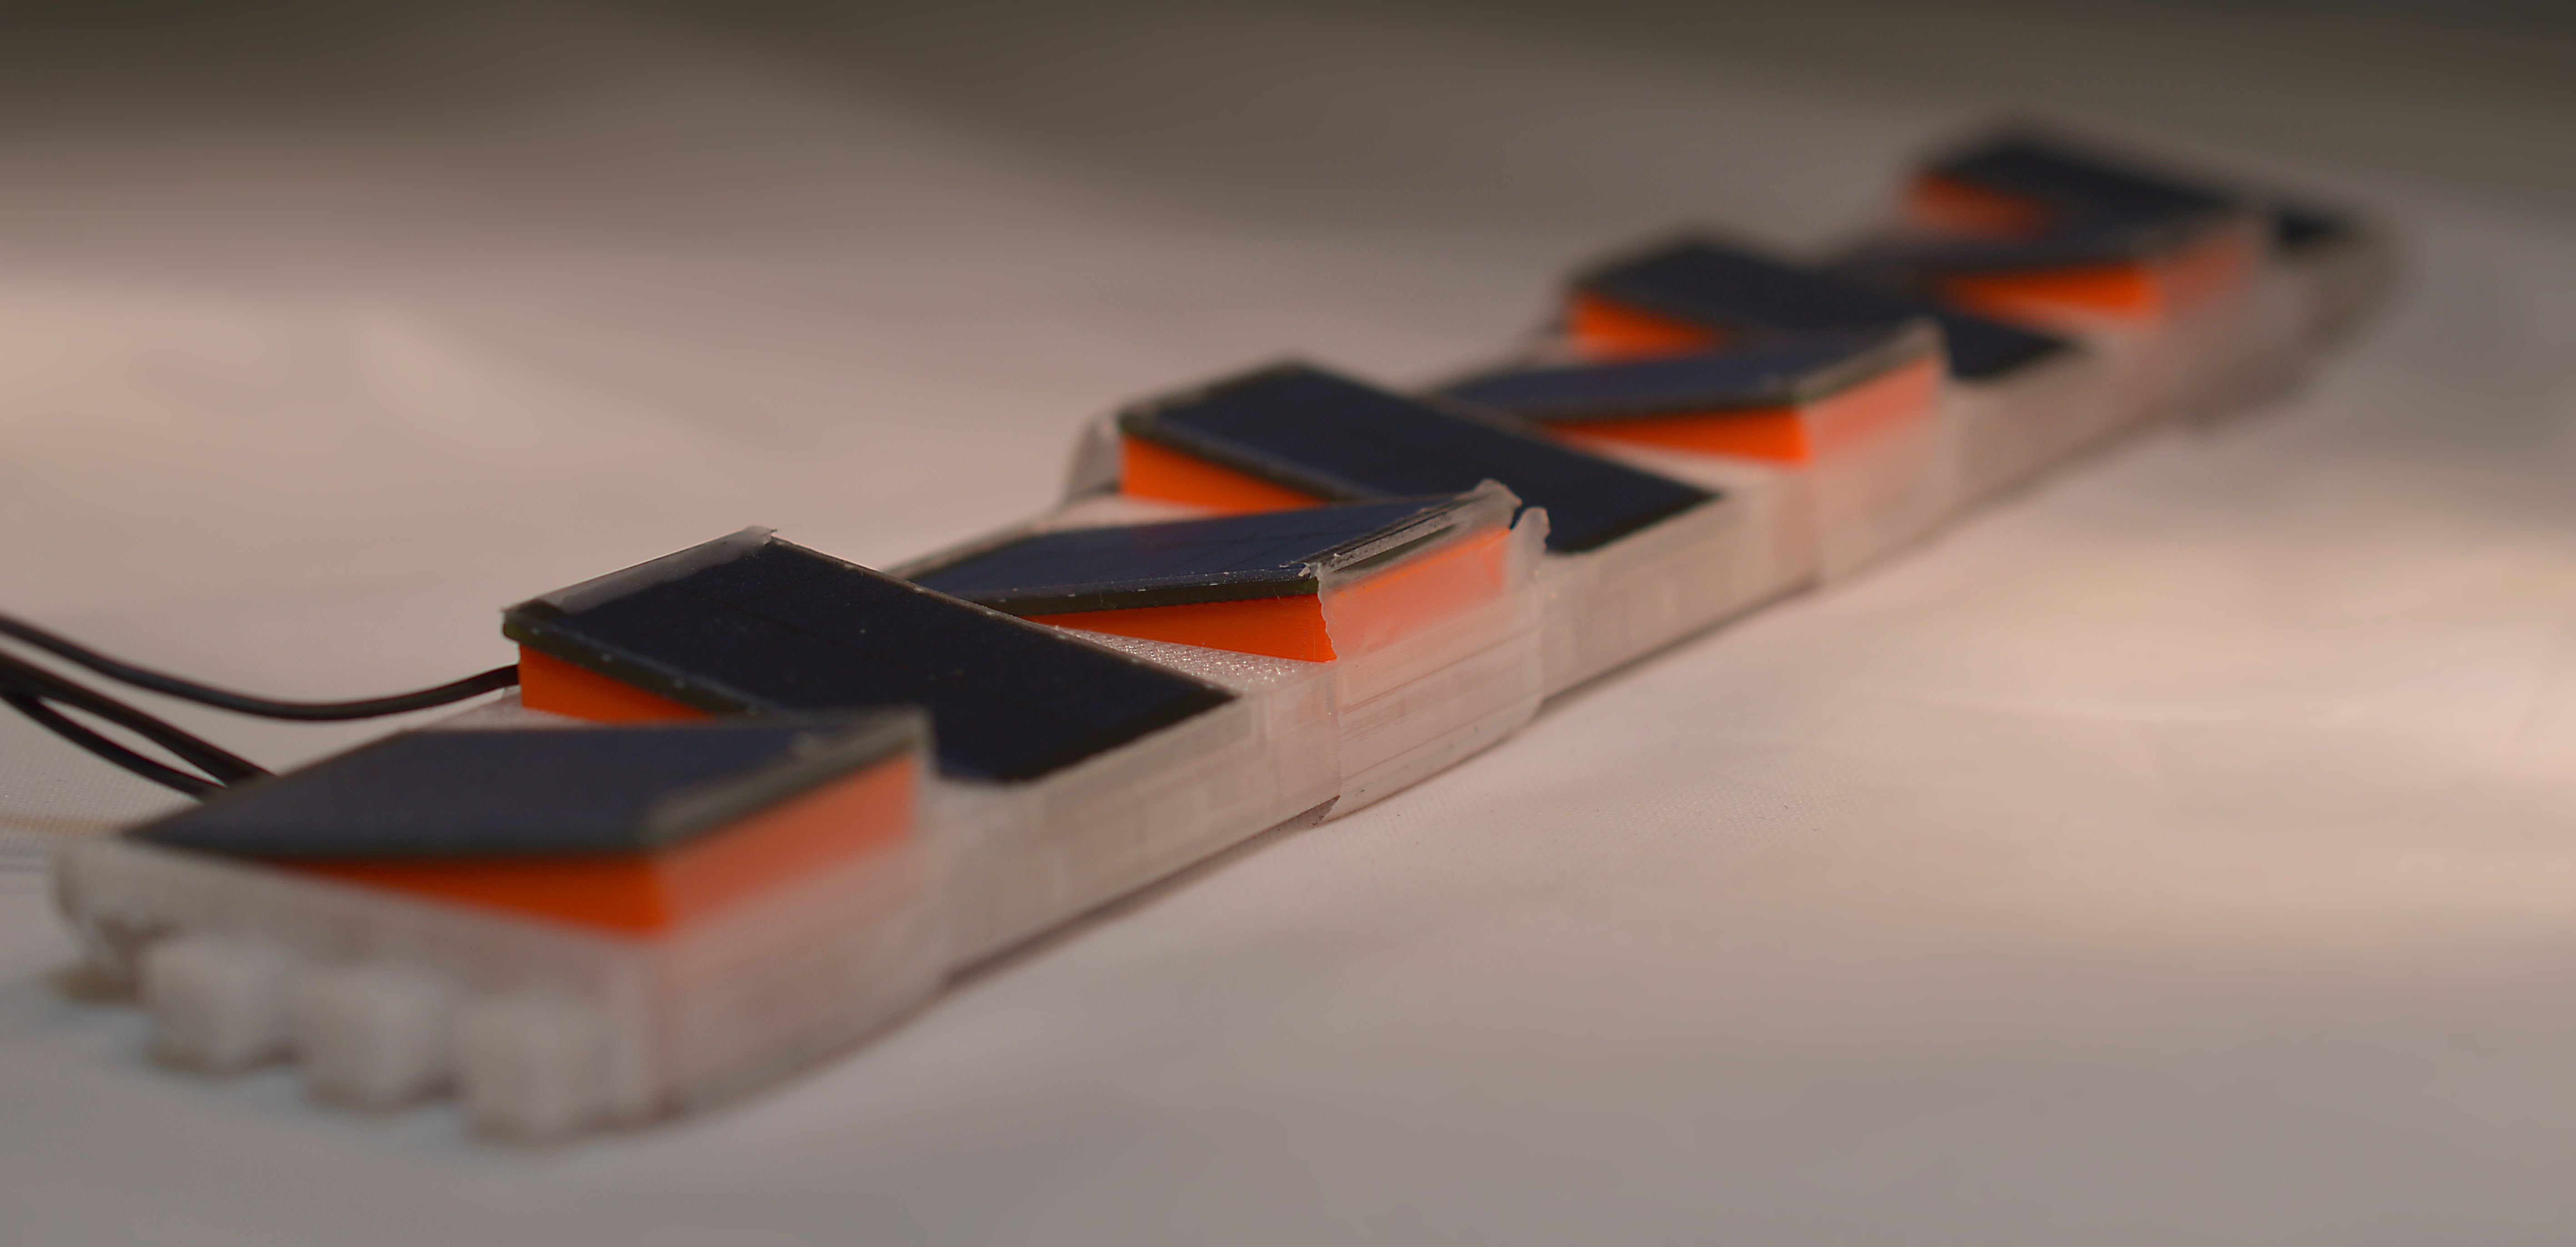
\includegraphics[width=\columnwidth]{figs/panels_lossy.jpg}
        \caption{3D printed solar panel enclosure with angled slots for solar energy harvesters.}
        \label{fig:mounting}
    \end{subfigure}%
    %
    \begin{subfigure}[b]{0.5\textwidth}
        \centering
        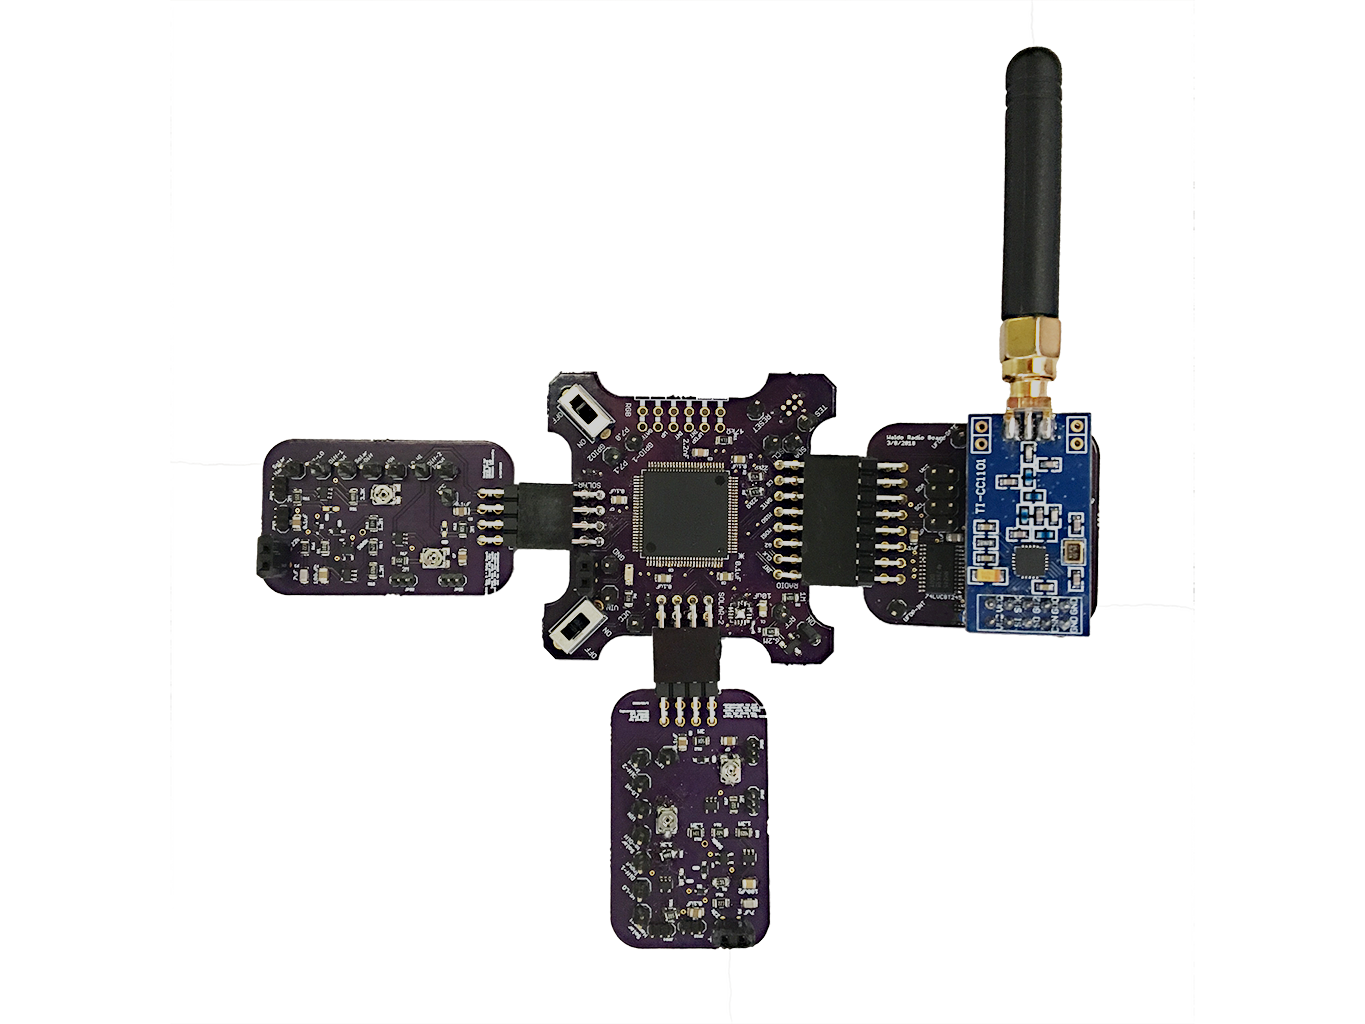
\includegraphics[width=0.75\columnwidth]{figs/board.png}
        \caption{ \sysname prototype PCB.}
        \label{fig:pcb}
    \end{subfigure}
    \caption{\sysname implementation \label{fig:prototype}}
\end{figure*}


We have implemented a prototype \sysname sensor for evaluating our approach, including custom hardware in the form of a Printed Circuit Board (PCB) (shown in \figref{fig:pcb}), firmware for managing the doorway sensing application, and a custom 3D printed doorway mounting system that holds the assembled PCB and solar panels in a slim profile \figref{fig:mounting}.

\noindpar{Hardware:} Our prototype hardware integrates four (4) RL-55x70 solar panels (70.00mm x 55.00mm) from Seeed and a custom printed circuit board~(PCB) held together by a 3D-printed plastic enclosure, detailed later in this section.
The prototype's hardware is composed of an MSP430FR6989 microcontroller from Texas Instrument's (TI) FRAM line of ultra-low-power processors.
The newest FRAM-based MSP430s have several advantages over previous models: lower sleep-mode currents, shorter wake-up latencies, and faster non-volatile FRAM.
Using the faster wake-up capabilities, \sysname is driven entirely by interrupts and remains asleep most of the time to conserve energy when not in use.
The solar panels are connected in two banks, where both of these banks are made up of two panels connected in parallel.
Both these banks are connected in series with each other to increase the harvesting voltage, allowing for greater volatility in voltage which makes it easier to recognize features of the signal.
This configuration provides enough current to power the circuit with sufficient voltage levels for detection, as well as powering the system.
The detector circuitry is made using nano-power comparators (TI TLV3691) and a passive RC filter network. The RC filter network is tunable using trim potentiometers pre-installation, or digital potentiometers in deployment.
The \sysname PCB also has a TI CC1101 radio for communication.
The hardware used in the \sysname prototype, shown in \figref{fig:pcb}, is not prohibitively expensive or obtrusive.
% solar panels are expensive: $14 for 8, device cost is 19.37
The total cost of the current prototype, including all PCB, parts, assembly costs, and solar panels is \$22.63 per unit if ordered in quantities of 1000. The distribution of the prototype costs are showed in Table \ref{tab:costbreakdown}.
The current prototype has several components that are meant to enable experimentation and testing (modular board design, jumpers, headers, test points, etc) -- a commercial version of \sysname will be dramatically cheaper and smaller.
\begin{table*}[t]
\footnotesize
\caption{Detailed breakdown of the \sysname prototype}
\label{tab:costbreakdown}
\begin{tabular}{@{}p{1.4in}llc@{}}
\toprule
\textbf{Components}          & \multicolumn{1}{r}{\textbf{Cost per individual unit}} & \multicolumn{1}{r}{\textbf{Unit Cost for 1000 units}} \\ \midrule
\textit{Solar Panels}       	& \$ 7.8	&  \$ 7	 \\
\textit{Microcontroller (MSP430FR6989)} & \$ 8.3	& \$ 4.71	\\
\textit{Components} & \$ 18.26	& \$ 8.72     \\ 
\textit{PCBs} & \$ 19.44	& \$ 2.2     \\ \midrule
\textit{Entire Waldo Prototype} & \$ 53.8	& \$ 22.63    \\ \midrule
\end{tabular}
\end{table*}

\noindpar{Firmware:}
The \sysname firmware implements the detection algorithm discussed in \secref{sec:system}.
Monitoring the interrupts from the detectors and deducing the direction of motion upon triggering are the main tasks of the system.
The firmware is designed to be ultra-low power, even in active mode, and has low computational complexity, offloading the bulk of the detection to the hardware circuits.
The \sysname firmware is composed of 398 lines of commented C code, compiling to a 2110 byte image. This code size comprises only 1.6\% of the available code space on the MSP430FR6989 (128KB), leaving ample room for implementing custom tasks, recognizers, or multiprogramming operating systems.

\noindpar{Mechanical Design:}
The 3D printed mounting system (shown in \figref{fig:mounting}) is made of PLA plastics and contains the PCB, solar cells, and necessary wiring connecting them.
\sysname's 3D printed enclosure measures \SI{13.2}{\centi\meter} by \SI{47.0}{\centi\meter} by \SI{1.0}{\centi\meter} at its thickest point. The enclosure provides a nesting place for the solar cells, pointing downward.
The angle of the solar cell slots is set such that some solar cells tend toward the entry, while the rest toward the exit.

All software, firmware, hardware schematics and layouts, and 3D printed mounting system will be made freely available at publication time.
